% TenantWall paper skeleton (IEEE conference format). Every "% WRITE:" comment is a prompt; replace it with your text.
% Build: pdflatex main && bibtex main && pdflatex main && pdflatex main
\documentclass[conference]{IEEEtran}
\usepackage{graphicx}
\usepackage{booktabs}
\usepackage{url}
\usepackage{listings}
\lstset{basicstyle=\ttfamily\footnotesize,breaklines=true,frame=single}
\begin{document}

\title{TenantWall: Attribute-Based Tenant Isolation and Denied-Access Alerting on AWS}
% Other title options: "Enforcing Multi-Tenant Isolation on Shared AWS Resources with ABAC and CloudTrail Alerting";
% "Tag-Based Isolation for Shared Cloud Resources: Design, Verification and Monitoring".

\author{\IEEEauthorblockN{[Author Name]}
\IEEEauthorblockA{{}[Department], [College]\\ {}[City], India\\ {}[email]}
\and
\IEEEauthorblockN{[Professor Name]}
\IEEEauthorblockA{{}[Department], [College]\\ {}[City], India\\ {}[email]}}

\maketitle

\begin{abstract}
% WRITE (150-200 words, last): problem (tenants sharing S3 and EC2 must not reach each other's data) ->
% approach (ABAC: tag-matched IAM policies plus explicit denies; CloudTrail -> CloudWatch -> SNS alerting) ->
% evaluation (N isolation tests, detection delay, cost) -> one-sentence result with numbers -> why it matters.
[Abstract.]
\end{abstract}

\begin{IEEEkeywords}
cloud security, multi-tenancy, attribute-based access control, AWS IAM, audit logging, intrusion detection
\end{IEEEkeywords}

\section{Introduction}
% WRITE: 1) shared cloud resources are cheap but risky; one misconfigured policy exposes a tenant's data.
% 2) role-per-tenant RBAC grows with every tenant; ABAC uses attributes (tags) so one policy serves all.
% 3) prevention is not enough: denied attempts should be detected and reported.
% 4) contributions, as a list:
\begin{itemize}
\item {}[Contribution 1: an ABAC policy design for tenant isolation on S3 and EC2, with explicit denies that survive later broad allows.]
\item {}[Contribution 2: an audit and alerting pipeline that reports denied cross-tenant access within minutes.]
\item {}[Contribution 3: an evaluation with N isolation tests, measured detection delay and cost.]
\end{itemize}
% End with a one-line roadmap of the paper.

\section{Background}
\subsection{Multi-tenancy in the cloud}
% WRITE: NIST definition of cloud computing and resource pooling \cite{nist800145}; isolation risks in shared clouds \cite{ristenpart2009}.
[Resource pooling and its isolation risks; sources: \cite{nist800145,ristenpart2009}.]
\subsection{RBAC and ABAC}
% WRITE: RBAC models \cite{sandhu1996}; ABAC definition and considerations \cite{nist800162}; unified ABAC model \cite{jin2012}.
% Explain why ABAC fits tenants: the tenant attribute on the principal must equal the tenant attribute on the resource.
[RBAC versus ABAC and why ABAC fits tenants; sources: \cite{sandhu1996,nist800162,jin2012}.]
\subsection{AWS IAM evaluation and CloudTrail}
% WRITE: explicit deny > allow > implicit deny \cite{awspolicyeval}; ABAC with principal and resource tags \cite{awsabac};
% CloudTrail management vs data events \cite{awsdataevents}.
[IAM evaluation order, ABAC in AWS and CloudTrail data events; sources: \cite{awspolicyeval,awsabac,awsdataevents}.]

\section{Threat Model}
% WRITE: assets (each tenant's objects and instances); attacker (a tenant, or anyone holding a tenant credential);
% trust boundary (IAM evaluation between tenant roles and shared resources); out of scope (AWS itself, account root compromise).
% Summarise the STRIDE table \cite{shostack2014} (see generated/security-lab-notebook.pdf) as one table:
[Assets, attacker, trust boundary and out-of-scope items; threats classified with STRIDE \cite{shostack2014}, summarised in Table~\ref{tab:stride}.]
\begin{table}[!h]
\caption{Threats and mitigations (STRIDE)}
\label{tab:stride}
\centering
\begin{tabular}{@{}ll@{}}
\toprule
Threat & Mitigation in TenantWall \\
\midrule
Spoofing & Roles with temporary credentials, MFA \\
Tampering & Explicit deny on tag changes; log validation \\
Repudiation & CloudTrail with S3 data events \\
Information disclosure & ABAC prefix and tag conditions; TLS only \\
Denial of service & Versioning; budget alarms \\
Elevation of privilege & No IAM write actions for tenant roles \\
\bottomrule
\end{tabular}
\end{table}

\section{Design}
% WRITE: architecture (Fig.~\ref{fig:arch}); the identity policy (tag and prefix matching); the explicit-deny policy;
% the bucket policy denying non-TLS requests; why denies are separate from allows. Show one short policy excerpt:
\begin{lstlisting}
"Condition": {"StringEquals": {
  "aws:ResourceTag/tenant": "${aws:PrincipalTag/tenant}"}}
\end{lstlisting}
\begin{figure}[t]
\centering
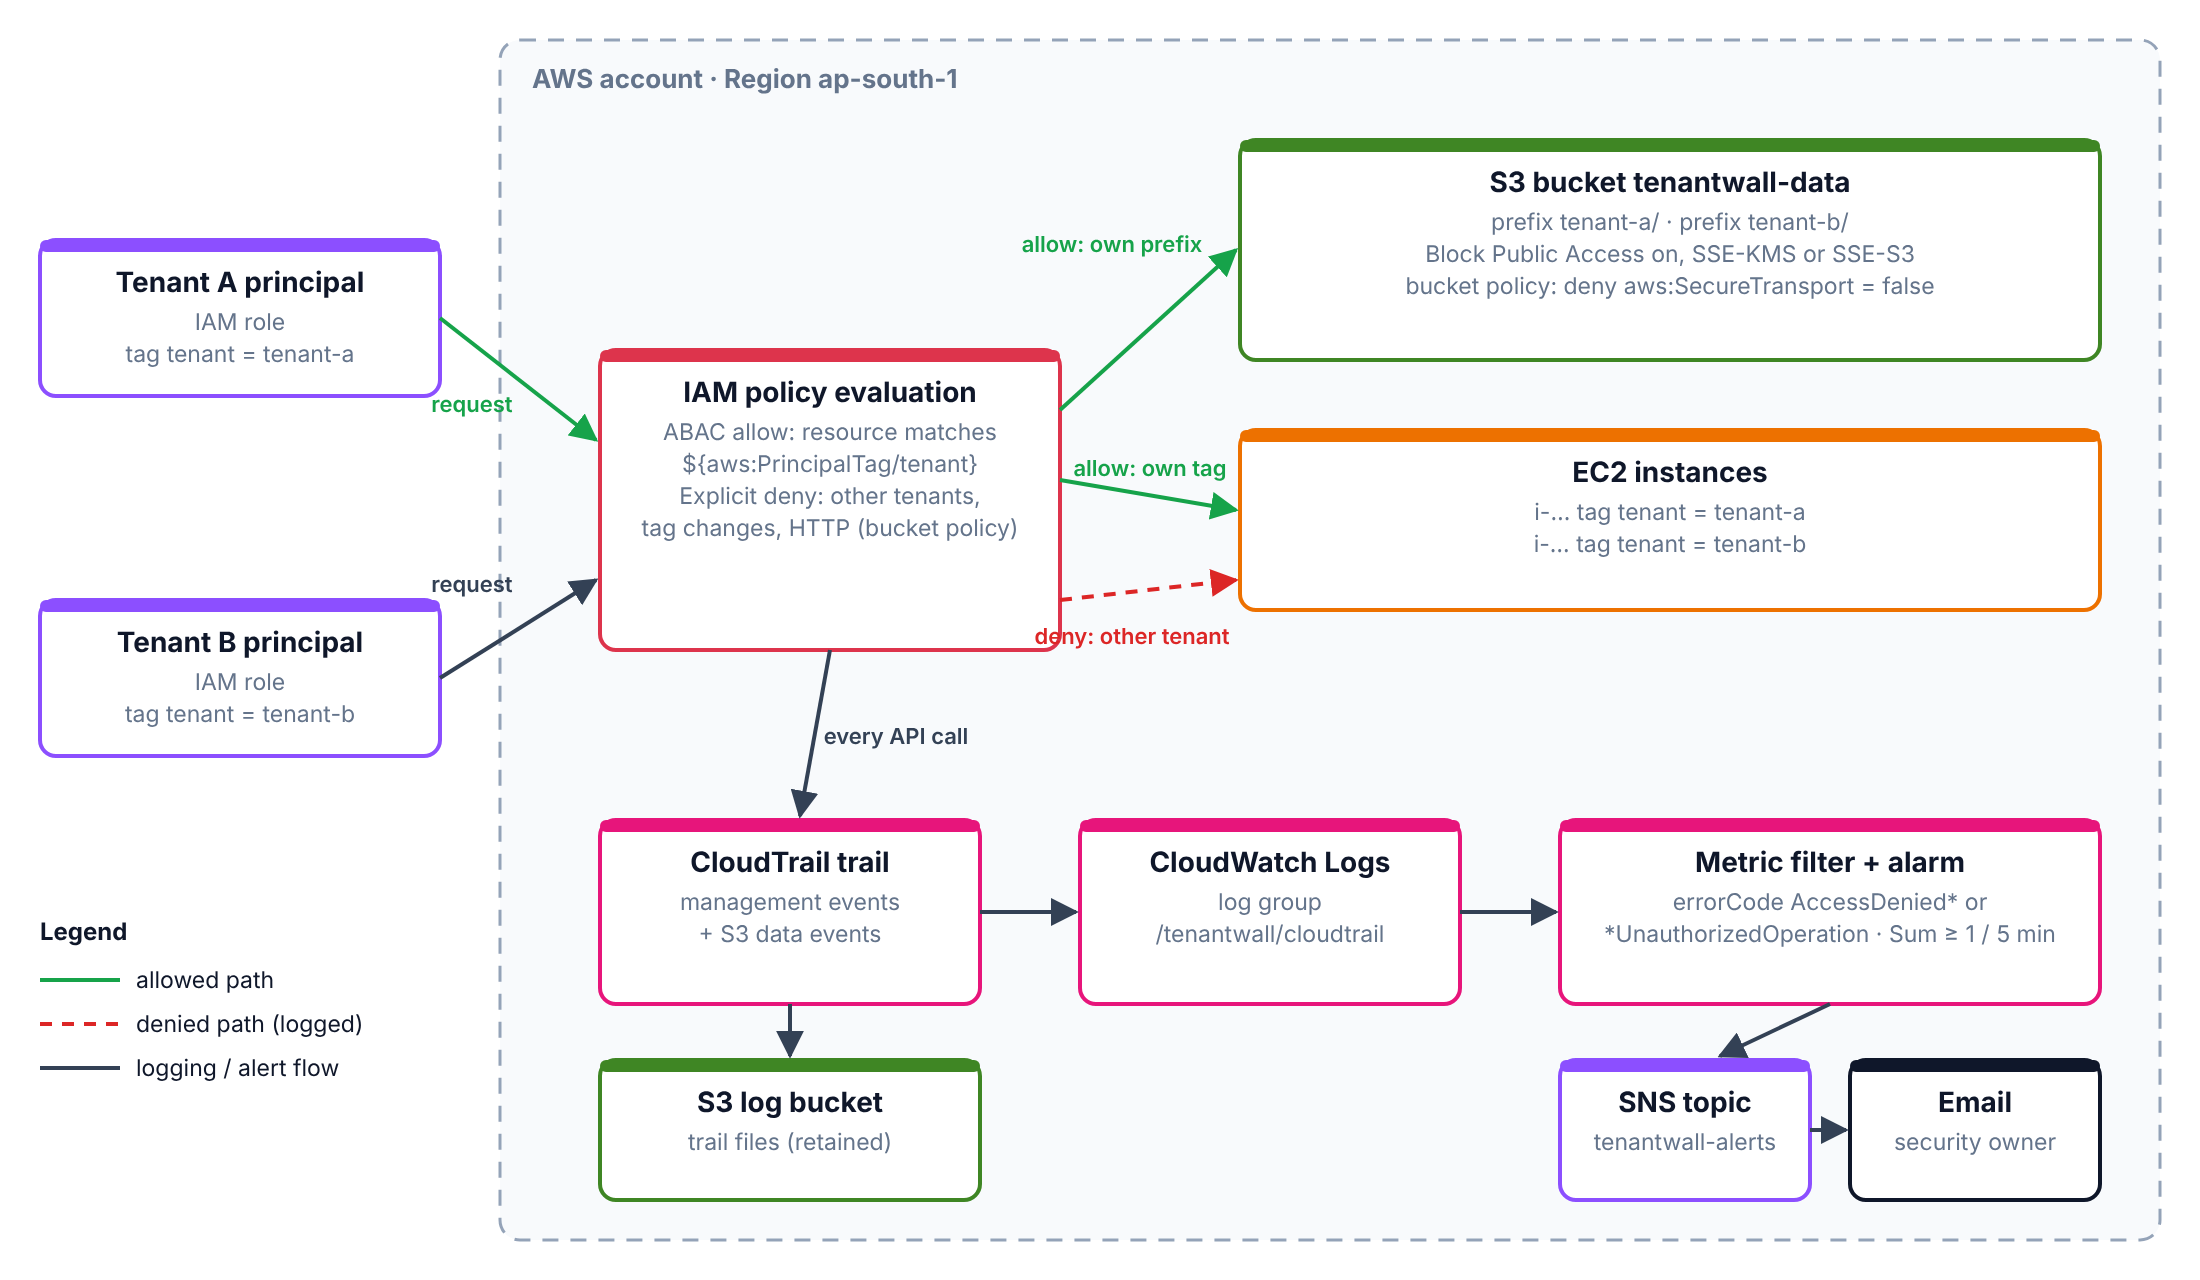
\includegraphics[width=\linewidth]{../architecture.png}
\caption{TenantWall architecture: tag-matched IAM evaluation and the CloudTrail $\rightarrow$ CloudWatch $\rightarrow$ SNS alerting path.}
\label{fig:arch}
\end{figure}

\section{Implementation}
% WRITE: region, services, how tenants and roles are created and tagged, the trail with S3 data events,
% the metric filter pattern and alarm settings (generated/tenantwall/alerting/), cost controls. Method flow: Fig.~\ref{fig:flow}.
\begin{figure}[t]
\centering
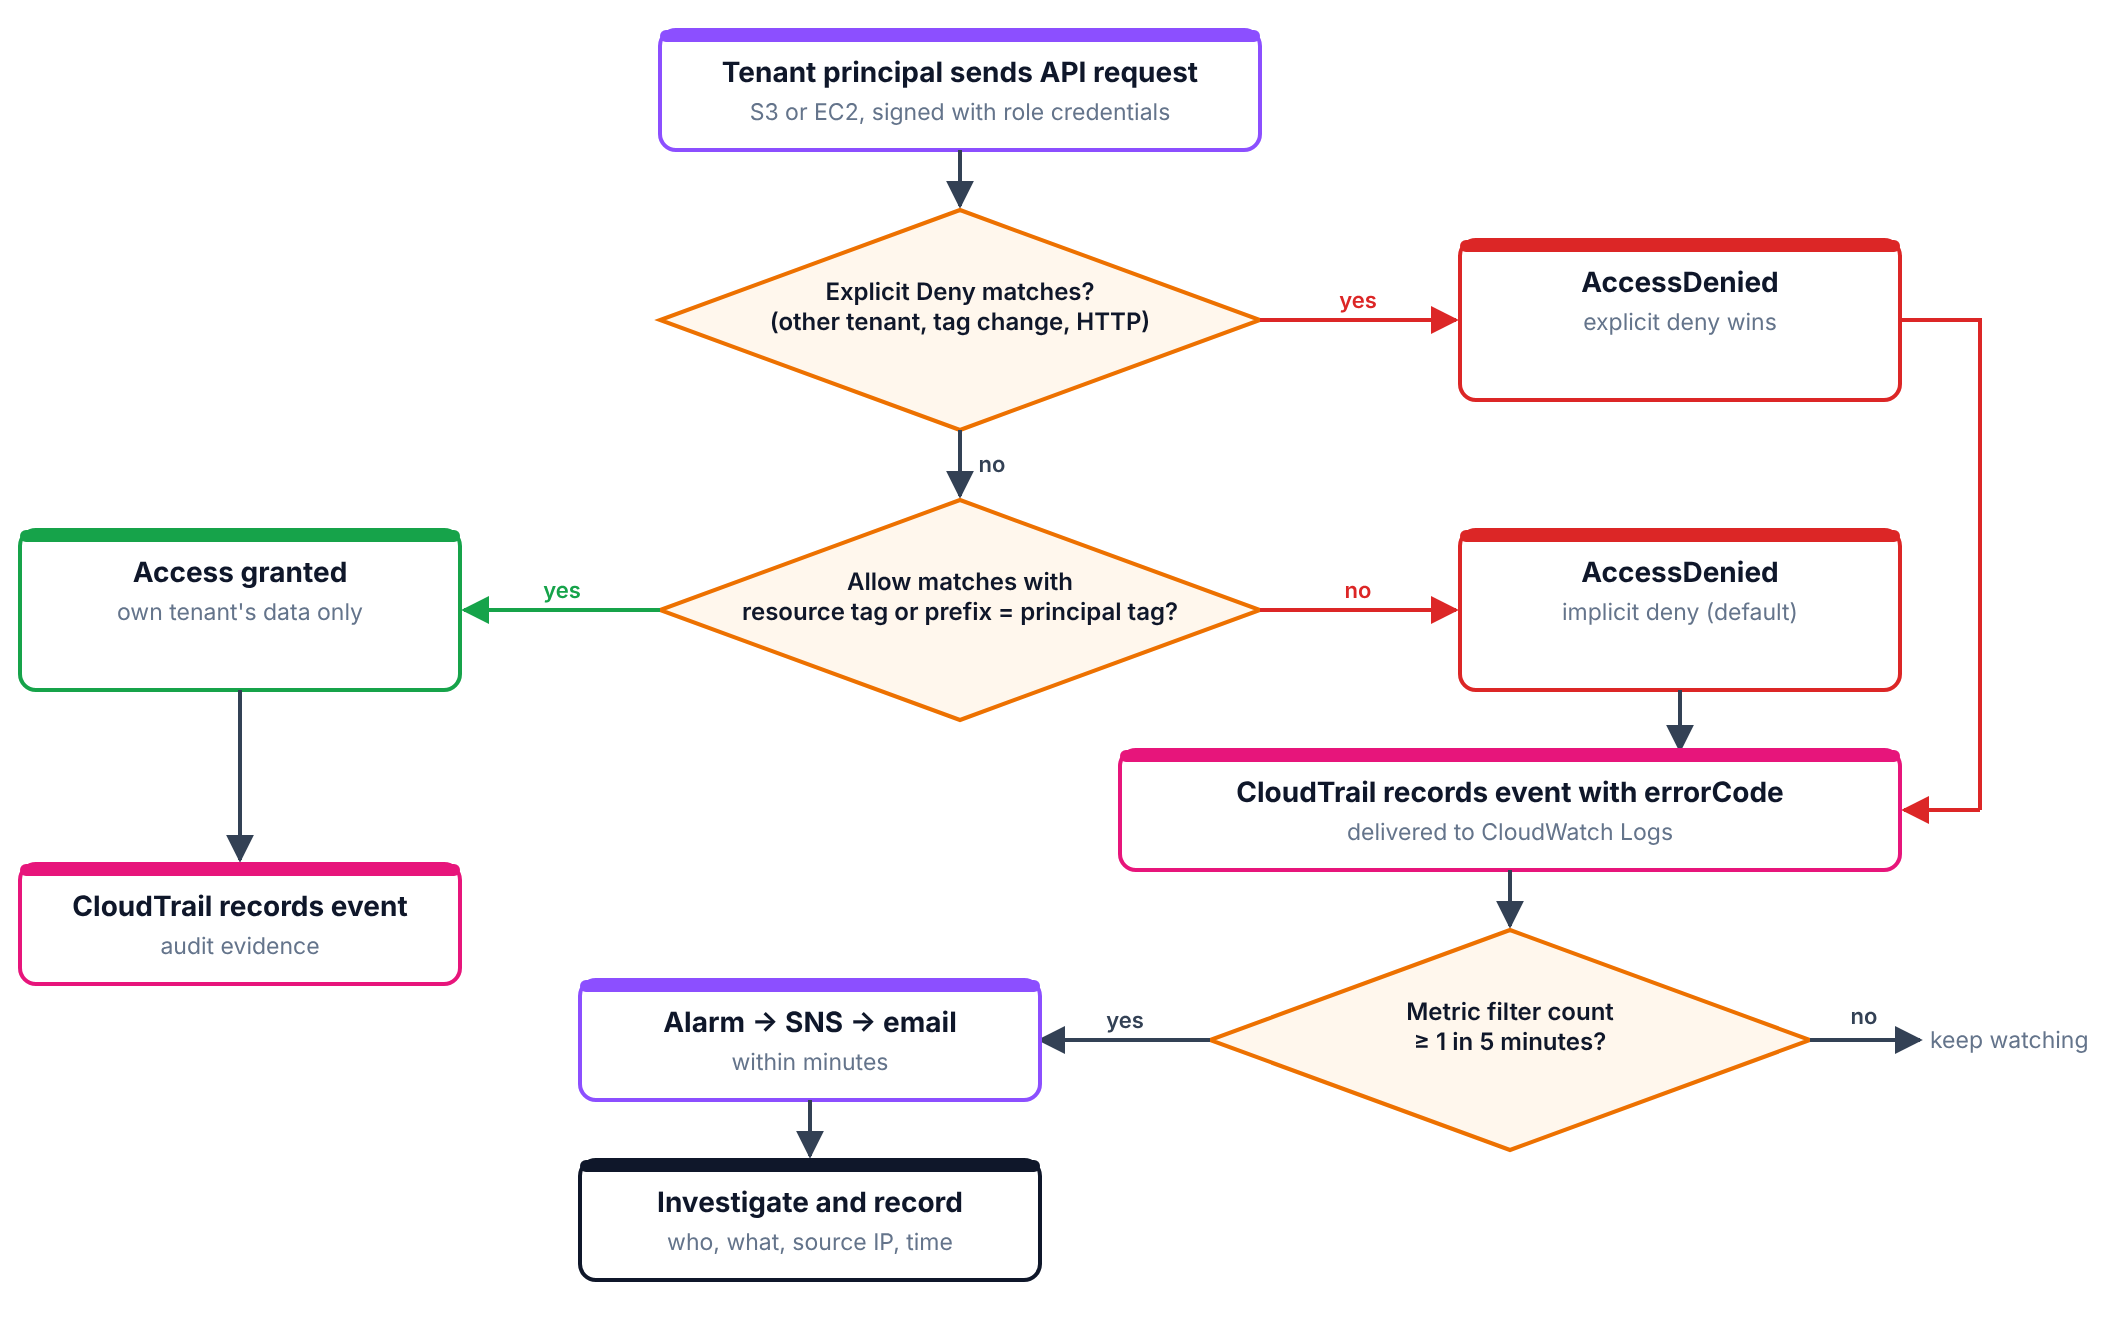
\includegraphics[width=\linewidth]{../flowchart.png}
\caption{Request evaluation and alerting method.}
\label{fig:flow}
\end{figure}

\section{Evaluation}
% WRITE: research questions (RQ1 isolation holds? RQ2 how fast are denied attempts reported? RQ3 cost and overhead?).
% Method: run the isolation test plan (generated/tenantwall-helpers.pdf) N times; record outcomes and alert delays.
\begin{table}[t]
\caption{Isolation test results}
\label{tab:results}
\centering
\begin{tabular}{@{}lccc@{}}
\toprule
Test & Expected & Observed & Alert (min) \\
\midrule
A reads B's object & Deny & [ ] & [ ] \\
A writes to B's prefix & Deny & [ ] & [ ] \\
A stops B's instance & Deny & [ ] & [ ] \\
A re-tags an instance & Deny & [ ] & [ ] \\
A reads own object & Allow & [ ] & -- \\
\bottomrule
\end{tabular}
\end{table}
% WRITE: detection delay as median and range over trials; false alerts seen; monthly cost of data events and logs.

\section{Discussion and Limitations}
% WRITE: tags as the trust anchor (who may set them); DescribeInstances has no resource-level control;
% CloudTrail delivery delay; scaling to many tenants; what would change for production.

\section{Related Work}
% WRITE: 1 paragraph each on cloud isolation \cite{ristenpart2009}, access-control models \cite{sandhu1996,jin2012,nist800162},
% and cloud audit/monitoring. Say how TenantWall differs (a concrete, tested design on one provider with alerting).

\section{Conclusion}
% WRITE: what was built, the measured results, and one line of future work (multi-account setups, automated policy testing).

\section*{Acknowledgment}
% WRITE: thank the professor and the department.

\bibliographystyle{IEEEtran}
\bibliography{refs}
\end{document}
